\documentclass[conference]{IEEEtran}
\IEEEoverridecommandlockouts
% The preceding line is only needed to identify funding in the first footnote. If that is unneeded, please comment it out.
\usepackage{cite}
\usepackage{amsmath,amssymb,amsfonts}
\usepackage{algorithmic}
\usepackage{graphicx}
\usepackage{textcomp}
\usepackage{xcolor}
\usepackage{soul}
\usepackage{biblatex} %Imports biblatex package
\addbibresource{bibliography.bib} %Import the bibliography file
\def\BibTeX{{\rm B\kern-.05em{\sc i\kern-.025em b}\kern-.08em
    T\kern-.1667em\lower.7ex\hbox{E}\kern-.125emX}}
    
    
\begin{document}


\title{Semantic Segmentation on Satellite Imagery (must change*)\\}
\author{\IEEEauthorblockN{Nancy Nigam}
\IEEEauthorblockA{\textit{Computer Science} \\
\textit{CIMS, NYU}\\
New York City, US\\
nn2163@nyu.edu}
\and
\IEEEauthorblockN{Aditya Upadhyaya}
\IEEEauthorblockA{\textit{Computer Science} \\
\textit{CIMS, NYU}\\
New York City, US\\
au2056@nyu.edu}
\and
\IEEEauthorblockN{Jorge Roldan}
\IEEEauthorblockA{\textit{Computer Science} \\
\textit{CIMS, NYU}\\
New York City, US\\
jlr9718@nyu.edu}
}
\maketitle

\begin{abstract}
\hl{Do abstract when we are done with everything else}
\end{abstract}

% ============================
\section{Introduction}
% ============================

% ============================
\section{Related Work}
% ============================


% ============================
\section{Datasets}
% ============================
% ----------------------------------------
\subsection{LandCoverNet Dataset}
% ----------------------------------------




\begin{table}[htbp]
\centering
\caption{LandCoverNet dataset}
\begin{tabular}{|p{1.8cm}|p{0.6cm}|p{1.6cm}|}
 \hline
 \multicolumn{3}{|c|}{\textbf{LandCoverNet Dataset Classes}} \\
 \hline
 \textbf{Class Name} & \textbf{Pixel Value}& \textbf{RGB Value} \\
 \hline
 Unkown & 0  & (0,0,0)\\ 
 \hline
 Water & 1  & (0,0,255)\\ 
 \hline
 Artificial & 2  & (136,136,136)\\ 
 \hline
 Natural & 3  & (209,164,109)\\ 
 \hline
 Snow/ice & 4 &  (245,245,255)\\ 
 \hline
 Wooddy & 5  & (214,76,43)\\ 
 \hline
 Cultivated & 7  & (24, 104, 24)\\ 
 \hline
 (Semi) Natural & 7  & (0, 255, 0)\\ 
 \hline
\end{tabular}
\label{landcovernet_dataset}
\end{table}

\subsection{Semantic Segmentation of Crop Type in Ghana Dataset}


\begin{table}[htbp]
\centering
\caption{Ghana Dataset}
\begin{tabular}{|p{2.2cm}|p{0.7cm}|p{1.6cm}|}
 \hline
 \multicolumn{3}{|c|}{\textbf{Crop Type in Ghana Dataset Classes}} \\
 \hline
 \textbf{Class Name} & \textbf{Pixel Value}& \textbf{RGB Value} \\
 \hline
  Unknown & 0  &  (0, 0, 0)\\ 
 \hline
  Ground nut & 1  & (80,0,165) \\ 
 \hline
  Maize & 2  & (255,204,0) \\ 
 \hline
  Rice & 3  & (0,244,244)\\ 
 \hline
  Soya bean & 4  & (105,105,105)\\ 
 \hline
  Yam & 5  & (255,255,102) \\ 
 \hline
  Intercrop & 6  & (255,153,153)\\ 
 \hline
  Sorghum & 7  & (127,222,209)\\ 
 \hline
  Okra & 8  & (222,127,219)\\ 
 \hline
  Cassava & 9  & (108,67,107)\\ 
 \hline
  Millet & 10  & (152,134,94)\\ 
 \hline
  Tomato & 11 & (99,228,150) \\ 
 \hline
  Cowpea & 12  & (99,176,228)\\ 
 \hline
  Sweet Potato & 13 & (255,186,186)\\ 
 \hline
  Babala Beans & 14  & (204,0,102) \\ 
 \hline
  Salad Vegetables & 15  & (102,51,0)\\ 
 \hline
  Bra and Ayolo  & 16  & (204,204,255)\\ 
 \hline
  Watermelon & 17  & (0,102,204)\\ 
 \hline
  Zabla & 18 & (255,0,255)\\ 
 \hline
  Nili & 19 & (102,0,204)\\ 
 \hline
  Kpalika & 20 & (141,51,117)\\ 
 \hline
  Cotton & 21 & (145,187,192)\\ 
 \hline
  Akata & 22 & (155,123,219)\\ 
 \hline
  Nyenabe & 23 & (193,0,76)\\ 
 \hline
  Pepper & 24 & (204,255,153)\\ 
 \hline
\end{tabular}
\label{ghana_dataset_class_table}
\end{table}

\subsection{LandCover.ai Dataset}



\subsubsection{Dataset Characteristics}
The LandCover.ai dataset consists of satellite imagery for semantic segmentation applications covering a region of Poland of a total area of 216.2 km$^2$ \cite{DBLP:journals/corr/abs-2005-02264}. The original dataset consists of 41 orthophoto tiles of 5 km$^2$ where 33 images and 8 images have a resolution of (9000 px x 9500 px) and (4200 px x 4700 px), respectively. \\ \indent
The authors of this dataset \cite{DBLP:journals/corr/abs-2005-02264} provided a script which we used to split these 41 images and their respective masks into 10,674 source and 10,674 masks images of (512 px x 512 px) resolution. These land cover of these images consist of agricultural areas (60 \%) and mixed forests (29.6 \%). \\ \indent



\subsubsection{Classes and RGB Mapping}
The name of the classes, their respective pixel value and RGB value are shown in table \ref{landcover_ai_classes}. The annotations were made manually by the authors using VGG  Image Annotator (VIA) \cite{dutta2019vgg}. According to \cite{DBLP:journals/corr/abs-2005-02264}, there are 12280 buildings (1.85 km$^2$), 72.02 km$^2$ of woodland, 13.15 km$^2$ of water, 3.5 km$^2$ of raods, and 125.75 km$^2$ of background, that is, the unknown class.

\begin{table}[htbp]
\centering
\caption{LandCover.ai Dataset}
\begin{tabular}{|p{1.2cm}|p{0.7cm}|p{1.6cm}|}
 \hline
 \multicolumn{3}{|c|}{\textbf{Landcover.ai Dataset Classes}} \\
 \hline
 \textbf{Class Name} & \textbf{Pixel Value}& \textbf{RGB Value} \\
 \hline
 Unknown & 0  & (0,0,0)\\ 
 \hline
 Building & 1  & (80,0,165)\\ 
 \hline
 Woodland & 2  & (255,204,0)\\ 
 \hline
 Water & 3  & (0,244,244)\\ 
 \hline
 Road & 4  & (105,105,105)\\ 
 \hline
\end{tabular}
\label{landcover_ai_classes}
\end{table}

% ============================
\section{Methodology}
% ============================
% ----------------------------------------
\subsection{Architectures}

For the purpose of our experiments, we leverage a U-Net network \cite{ronneberger2015unet}. U-Net is a fully convolution neural network used extensively for image segmentation. It involves encoder and decoder components connected with skip connections. For the classification model that serves as our encoder and extracts features of different spatial resolution, we use a ResNet architecture \cite{DBLP:journals/corr/HeZRS15}. As part of our ablation study, we also review a U-Net++ network \cite{DBLP:journals/corr/abs-1807-10165} which consists of convolution layers on skip pathways.
% ----------------------------------------

% ----------------------------------------
\subsection{Evaluation Metrics}
% ----------------------------------------
 The lead evaluation metric for us is the Jaccard Index, also known as Intersection over Union (IoU).
\begin{equation*}
    IoU=\frac{target \cap prediction}{target \cup prediction}
\end{equation*}

In addition to IoU, we also capture Pixel Accuracy, Precision, and Recall. High pixel accuracy (the number of pixels classified correctly) doesn't always imply good segmentation results, especially in cases of class imbalance. This is true in our case since the 'woodland' class dominates all other classes.

% ============================
\section{Setup and Experiments}
% ============================

\subsection{Setup}
Our entire data augmentation, training, and prediction pipeline is implemented on the PyTorch framework (cite) and we use the NVIDIA V100 GPU (cite) to speed up our computations. The SMP library (cite) provides us segmentation models with pre-trained backbones. 
\\
\\Typically, neural network initialized with weights from a pre-trained network shows better performance and for our purposes, we initialize our ResNet encoder with ImageNet (cite) weights. The encoder depth is kept at a constant value of 5 throughout the scope of our experiments. 

\subsection{Hyperparameters}
Our seed dataset is divided into train-validation-test with a ratio of 80:10:10. A batch size of 32 works best for our use-case and we keep this value constant throughout. The Adam optimizer is our choice for all our experiments as it helps us converge faster and we apply a softmax activation after the final convolution layer. A bit of fine-tuning helps us arrive at a starting learning rate of $1\text{e-}4$ for our StepLR with a multiplicative factor of 0.1 every 15 epochs. Finally, the choice for our loss function is the Focal Loss as it helps us address class imbalance. We do consider other loss functions (Cross Entropy Loss and Dice Loss) and we discuss this in detail in the next section.
\subsection{Experiments}
We conduct a variety of experiments across multiple configurations of our pipeline and we discuss them in detail.

\subsubsection{Dataset Challenges}
Datasets in their raw form pose a serious challenge due to multiple factors. For instance, the Ghana Dataset (cite) comprises of low-res images, class imbalance, and high cloud cover. On the other hand, the LandCoverNet dataset excels in terms of image quality and adequate labels for each class, but it comes up short when it comes to cloud cover. Figure 1 illustrates the results of one such experiment we conduct on this dataset.

\subsubsection{Loss Functions} As part of this study, we do a comparative analysis of three loss functions - Focal, Dice, and Cross Entropy. We plug a ResNet18 encoder (with pre-trained ImageNet weights) in our U-Net network. Training is done for a total of 40 epochs. Fig 1 shows the predicted masks when we oversample the woodland representation (on an already unbalanced dataset).

\begin{figure*}
    \centering
    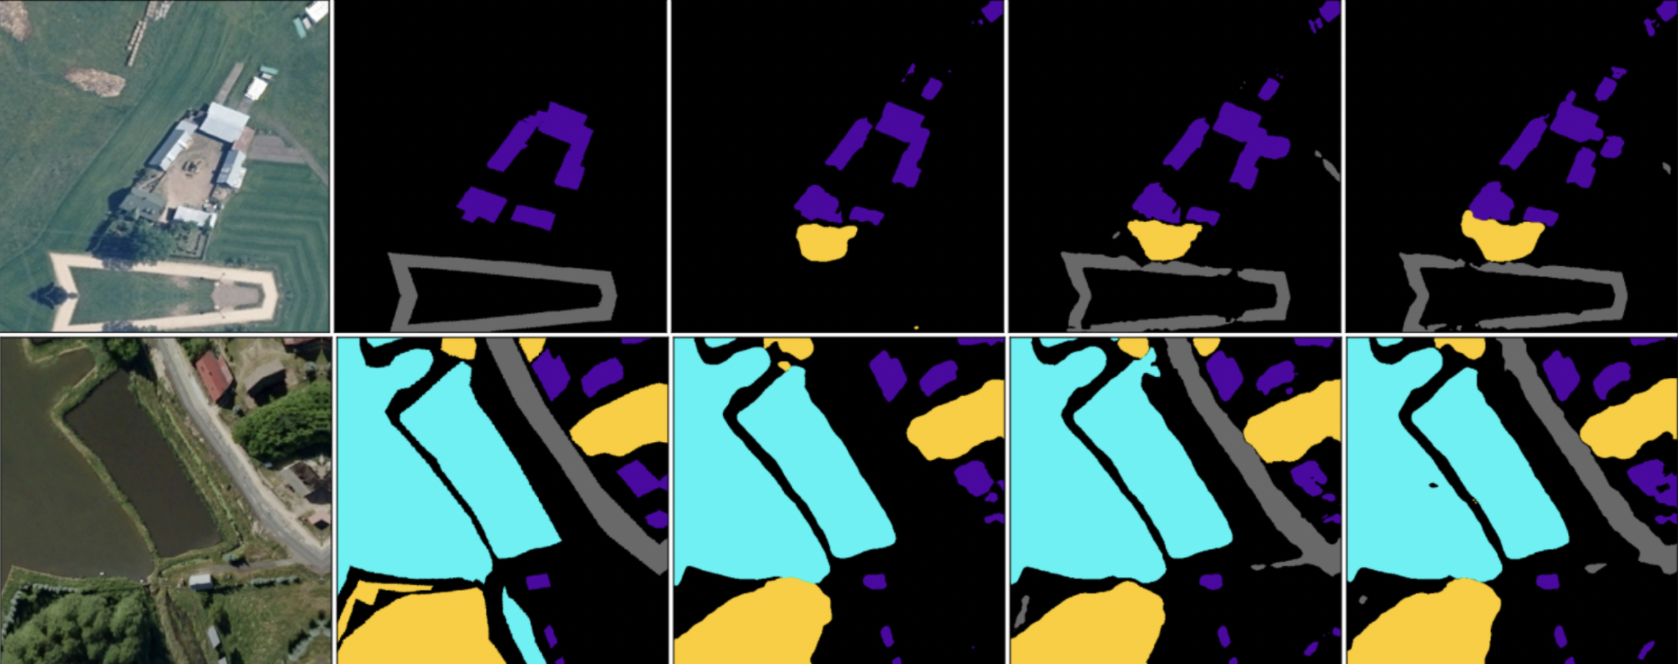
\includegraphics[width=\textwidth]{no-roads-loss/2-images.png}
    \caption{Prediction on a highly-imbalanced dataset with a U-Net network on a ResNet18 encoder. The first column contains the actual images, the second column represents the target mask, the third, fourth, and fifth columns represent the predicted mask with Dice, Focal, and Cross Entropy Loss respectively. Dice Loss(third columns) fails to detect the minority class (roads) in a lot of samples}
\end{figure*}

Fig. 2 shows the predicted masks on our actual dataset. Fig 3 and Fig 4 depict the progression of IoU and F-Scores respectively over the training iterations.
\begin{figure*}
    \centering
    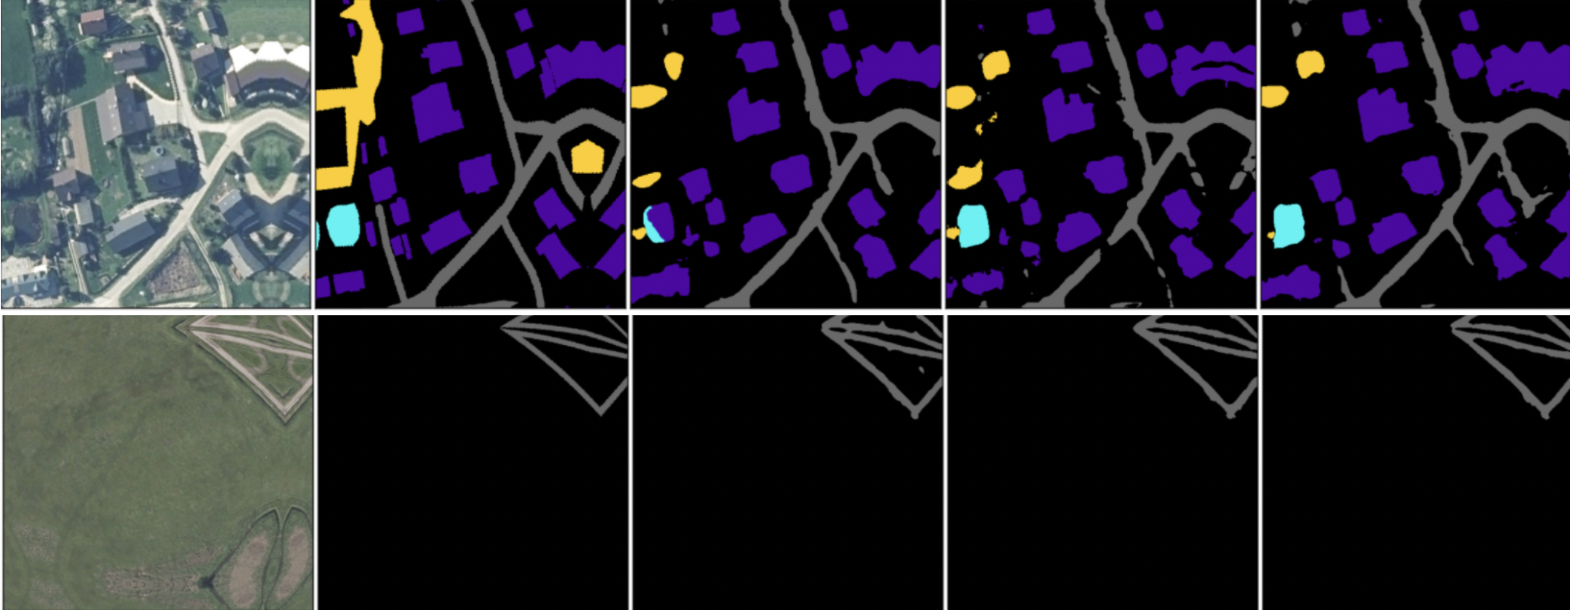
\includegraphics[width=\textwidth]{roads-losses/with-roads.png}
    \caption{Prediction on a more balanced dataset with a U-Net network on a ResNet18 encoder. The first column contains the actual images, the second column represents the target mask, the third, fourth, and fitth columns represent the Predicted Mask with Dice, Focal, and Cross Entropy Loss respectively}
\end{figure*}

\begin{figure}[!hb]
    \centering
    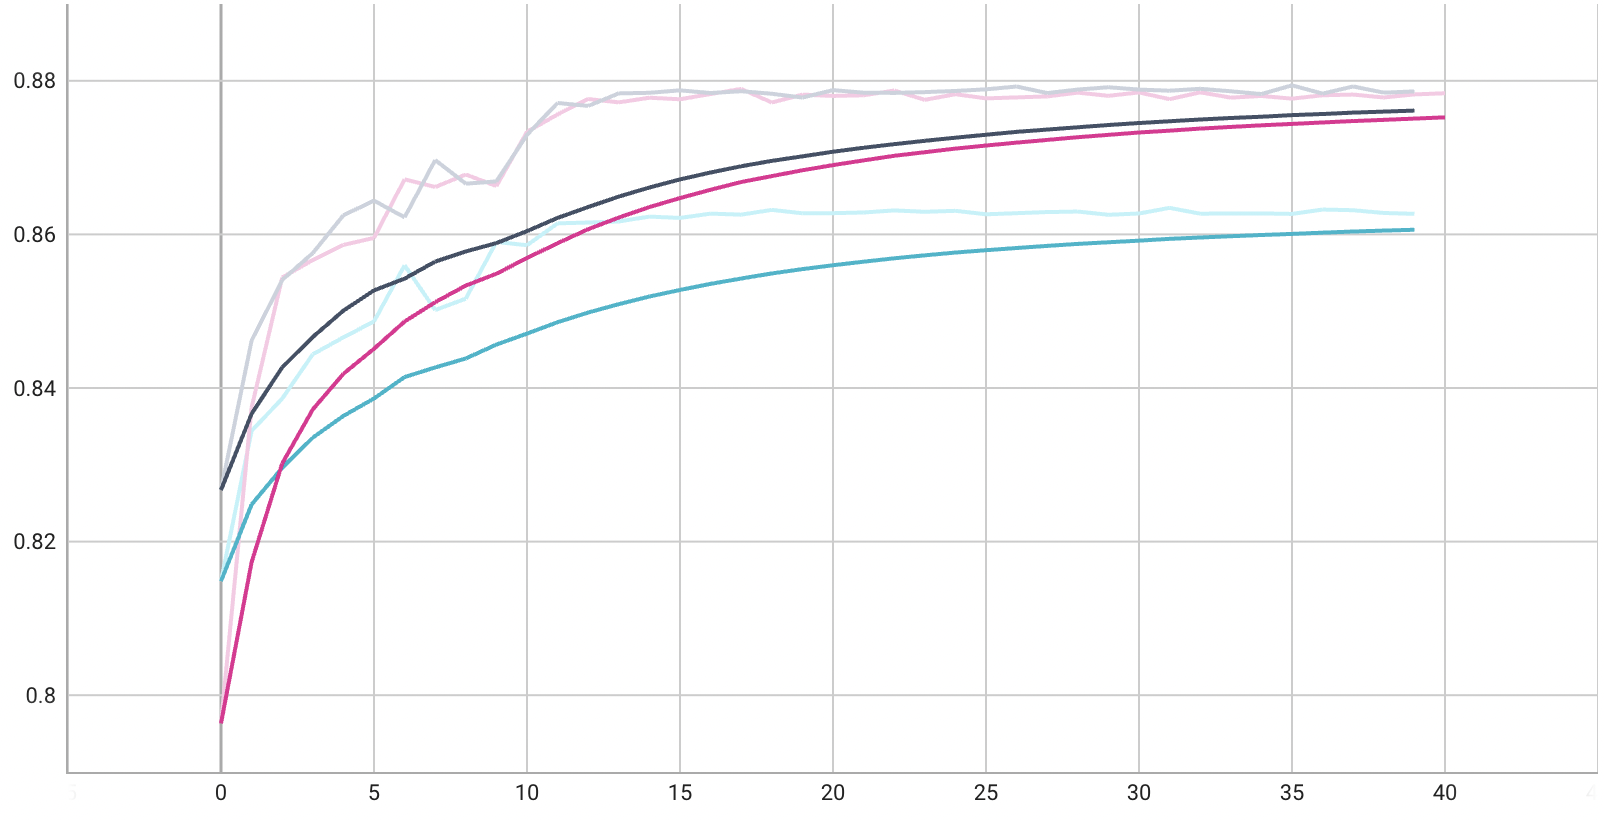
\includegraphics[width=80mm, scale=2.5]{roads-losses/three-losses-iou.png}
    \caption{Progression of IoU Scores over 40 epochs for Focal Loss (Magenta), Dice Loss (Teal), and Cross Entropy Loss (Gray). U-Net network having a ResNet18 encoder pre-trained with ImageNet weights. The dataset doesn't have an imbalance. }
\end{figure}

\subsubsection{Number of Layers in the Encoder} The intent of this experiment is to observe the effect of the depth of a net work. ResNet18, Resnet35, and Resnet50 are our encoder choices and we start with pre-trained ImageNet weights. Focal Loss measures the difference between the actual values and our estimated values. We train for a total of 50 epochs and the results are shown in Fig10 and IoU progression is shown in Fig11.

\subsubsection{U-Net vs U-Net++} We now replace our original U-Net network with U-Net++. We use ResNet34 as our encoder with pre-trained ImageNet weights. Again, Focal Loss is our choice for the loss function and we train for a total of 50 epochs. 


% ============================
\section{Results}
% ============================
\begin{enumerate}
    \item Focal Loss performs the best in scenarios of data imbalance. On the other hand, IoU values remain comparable between the three loss functions when the dataset is slightly balanced.
    \item ResNet50 performs best vs 18 and 34
    \item U-Net++ provides a better.
\end{enumerate}
% ============================
\section{Conclusion}
% ============================

\printbibliography %Prints bibliography


\end{document}
